\documentclass[12pt]{article}
\usepackage[utf8]{inputenc}
\usepackage{amssymb,amsmath,amsfonts,eurosym,geometry,ulem,caption,color,xcolor,multicol,setspace,sectsty,comment,footmisc,caption,natbib,pdflscape,subfigure,array,hyperref,verbatim,mathpazo,longtable,ntheorem,siunitx}
%\usepackage[normalem]{ulem}
\usepackage[pdftex]{graphicx}
\graphicspath{{Imagens/}}
\usepackage{fullpage}
\usepackage{indentfirst}
\usepackage{changepage}

%\setlength{\pdfpagewidth}{8.5in} \setlength{\pdfpageheight}{11in}
%\setlength{\textheight}{8.5in} \setlength{\topmargin}{0.0in}
%\setlength{\headheight}{0.0in} \setlength{\headsep}{0.0in}
%\setlength{\leftmargin}{0.5in}
%\setlength{\oddsidemargin}{0.0in}
%\setlength{\parindent}{2em}
%\setlength{\parskip}{\baselineskip}%
%\setlength{\textwidth}{6.5in}
%\linespread{1.6}
\newcommand*{\captionsource}[2]{%
  \caption[{#1}]{%
    #1%
    \\\hspace{\linewidth}%
    \textbf{Source:} #2%
  }%
}
\newcommand{\horrule}[1]{\rule{\linewidth}{#1}} % Create horizontal rule command with 1 argument of height

\onehalfspacing
\newtheorem{theorem}{Theorem}
\newtheorem{corollary}[theorem]{Corollary}
\newtheorem{proposition}{Proposition}
\newenvironment{proof}[1][Proof]{\noindent\textbf{#1.} }{\ \rule{0.5em}{0.5em}}

\newtheorem{hyp}{Hypothesis}
\newtheorem{subhyp}{Hypothesis}[hyp]
\renewcommand{\thesubhyp}{\thehyp\alph{subhyp}}

\newcommand{\red}[1]{{\color{red} #1}}
\newcommand{\blue}[1]{{\color{blue} #1}}

\newcolumntype{L}[1]{>{\raggedright\let\newline\\arraybackslash\hspace{0pt}}m{#1}}
\newcolumntype{C}[1]{>{\centering\let\newline\\arraybackslash\hspace{0pt}}m{#1}}
\newcolumntype{R}[1]{>{\raggedleft\let\newline\\arraybackslash\hspace{0pt}}m{#1}}

\geometry{left=1.2in,right=1.2in,top=1.2in,bottom=1.2in}
\begin{document}
	
	\begin{titlepage}
		\title{Macroprudential Policies and Capital Structure: Evidence from Multinationals \thanks{Research Master Thesis under supervision of Prof. Dr. Harry Huizinga and Dr. Louis Raes}}
		\author{Lucas Avezum}
		%\author{Lucas Avezum\thanks{abc} \and \and Harry Huizinga\thanks{abc} \and Louis Raes\thanks{abc}}
		\date{\today}
		\maketitle
		\begin{abstract}
			\noindent This paper studies how macroprudential policies, specifically reserve and capital requirements, relate to non-financial firms' capital structure. We first present a model where macroprudential instruments affect banks' costs which in turn are transmitted to firms' leverage through their cost of debt. Using a firm-level dataset of multinationals hosted in 37 countries we are able to identify domestic and international effects. The empirical results show that tighter capital requirements reduce firms' leverage while multinationals have an extra incentive to lower debt levels in subsidiaries hosted in countries with relative higher reserve requirements. Moreover, the domestic effect is found to be stronger for riskier firms.  \\
			\vspace{0in}\\
			%\noindent\textbf{Keywords:} key1, key2, key3\\
			\vspace{0in}\\
			%\noindent\textbf{JEL Codes:} key1, key2, key3\\
			
			\bigskip
		\end{abstract}
		\setcounter{page}{0}
		\thispagestyle{empty}
	\end{titlepage}
	\pagebreak \newpage
	
	
	
	
	\doublespacing
	
	
	\section{Introduction} \label{sec:introduction}
	As \cite*{NBERw22735} documented, the mandate of central banks has expanded considerably. Triggered mostly by the 2008 financial crisis, financial stability is perceived by many central banks as a goal together with price stability. To achieve the former, several macroprudential instruments were included or extended in entral bankers' toolboxes. However, the authors also note that the extent in which these policies will be used in the future is still unclear. Given its early stage, the effectiveness and externalities of macroprudential instruments have yet to be properly evaluated. This paper studies how macroprudential policies, specifically reserve and capital requirements, relate to non-financial firms' capital structure. Domestic and international effects are evaluated and found to be statistically and economically significant. 
	
	Multinationals take into account tax and non-tax factors when deciding their optimal financial structure and how to allocate debt through their subsidiaries. Apart from the expected bankruptcy and agency costs associated to debt, changes in the cost of debt might also impact firms' capital structure. For instance, a booming credit market in one country may lead to higher leverage at subsidiaries hosted in this country, as the multinational will take advantage of better financing conditions (domestic effect). Given an optimal leverage level for the multinational, subsidiaries of this corporate group hosted at other countries should reduce external financing relative to purely domestic firms at the same country, otherwise the indebtedness of the multinational would no longer be at the optimal level (international effect). As macroprudential instruments aim at smoothing credit markets, to the degree of their domestic effectiveness, international spillovers in the form of debt shifting are expected. 
	
	We first present a model of the multinational corporation's optimal capital structure, based on \cite*{huizinga2008capital}, that considers the trade-off between the tax advantages of debt versus the bankruptcy and agency costs related to it. We add to the standard theory the transmission of macroprudential policies to firms' cost of debt. Our model predicts for any establishment of the multinational that: tight local macroprudential policies and differences between local and foreign macroprudential policies (that is, local policy is tighter) to decrease leverage; local tax rate and differences between local and foreign tax rates (that is, higher local tax rate) to be positively associated with leverage; and the interaction between macroprudential instruments and the tax rate to be positively correlated with leverage. The last effect channel is due to a higher debt tax shield that comes with a higher cost of debt.
	
	Empirical evidence on the impact of macroprudential policies on firms' capital structure is provided for a sample of 102,544 firms hosted in 37 countries and belonging to 29,453 multinational corporate groups. Our identification strategy relies on two aspects of our data: first, firm-level data mitigate endogeneity concerns as the leverage level of a non-financial firm is not considered for decisions on capital and reserve requirements; and second, with ownership information we can track multinational groups and use variations in prudential tools that are not common to all firms within the group. Thus, we can control for unobservables on the demand side and common shocks at the country-level that could be correlated to macroprudential policies' changes. In some specifications we also add an interaction term between the macroprudential policies indexes and firms' riskiness that we proxy by their volatility of profits. Riskier firms face worse credit conditions, hence we expect this interaction term to be negatively associated to firms' leverage.
	
	Overall, the empirical results show that tighter capital requirements reduce firms' leverage while multinationals have an extra incentive to lower debt levels in subsidiaries hosted in countries with relative higher reserve requirements. Considering the interaction with firms' riskiness, the domestic effect of one tightening measure in capital requirements is estimated to lower leverage by 3.6\% on average, a sizable impact given that the average leverage level in our sample is 7\% higher relative to the level in 2007.
	
	Research on the effects of prudential policies has increased considerably after the 2008 financial crisis. Several authors rely on cross-country aggregate data to study the relationship between macroprudential policies and financial indicators. \cite*{cerutti2015use} introduces a dataset containing the usage of 12 macroprudential policies at 119 countries from 2000 to 2013. They document that prudential instruments are mostly used in developing countries where they also appear to be more effective. Among their findings, borrower-related policies, such as limits on loan-to-value and debt-to-income ratios are associated with reductions in credit growth and house prices. The author also provide an extensive review of the literature on macroprudential policies. 
	
	A second line of studies provides micro-level evidence. With loan-level data \cite*{jimenez2012macroprudential} study the  effects of capital buffers in Spain. The authors show that counter-cyclical capital buffers are effective in both directions: reduce credit growth in booming times while helps sustain credit in recessions. \cite*{aiyar2014does} find lending to leak through foreign branches following an increase in capital requirements to regulated banks. Their work shows that capital requirements in UK were effective in curbing lending for regulated banks, but the leakage is substantial. Most studies in this second group of the literature focus on few instruments, on the bank or housing sectors and are restricted to one country. An exception is the work by \cite*{ayyagari2017credit} that uses firm-level data to relate macroprudential policies across 119 countries to firms' debt growth. They find that the effectiveness of prudential tools at smoothing credit depend on the firm's location (emerging or developed country), size, debt maturity and the type of instrument (borrower-target or financial institution target). 
	
	Our work is closely related to the series of papers developed under the International Banking Research Network (IBRN) 2015 initiative. \cite*{buch2017cross} summarize the methodology and provide a meta-study. The authors also rely on multinational relationships to identify international spillovers. However, their analyses focus on banking loans, while we study changes in firms' capital structure. Among their findings, the effects of prudential tools are heterogeneous on type and location. On average, the economic significance of international spillover is found to be small.  
	
	Finally, this paper also builds on the capital structure literature. Many papers study the determinants of firms' leverage, both theoretical and empirically. \cite*{titman1988determinants} and more recently, \cite{oztekin2015capital} provide an overview of and test the different proposed capital structure's determinants. Following the literature's findings, we control for several firm characteristics such as, profitability, tangibility, growth opportunities, firm size and riskiness. However, to robustly  identify the effect of macroprudential policies on firms' capital structure we go beyond and control for time varying country and multinational characteristics. Supporting our empirical strategy, \cite*{booth2001capital} show the importance of specific country factors to account for differences in leverage across firms hosted in different countries. 
	
   The main contribution of the paper is to show that macroprudential policies, that is, capital and reserve requirements affect firms' leverage. Two important transmission channels of macroprudential instruments are identified. On one hand, the domestic effect helps central bankers in their new policy goal of sustaining financial stability as it curbs excessive leverage of firms. On the other hand, the finding of international spillovers, albeit small, points towards the necessity of further policy coordination among countries.        
	
	The paper proceeds as follows: section \ref{sec:model} presents the model and section \ref{sec:data} describes the data. The empirical strategy and hypothesis are described in section \ref{sec:strategy} while the results are discussed in section \ref{sec:result}. Section \ref{sec:robustness} presents some extensions and Section \ref{sec:conclusion} concludes. 
	
		\section{Model} \label{sec:model}
	In this section we present a model of the optimal capital structure of multinationals based on \cite{huizinga2008capital} who consider tax and non-tax factors in the firms' decision problem. We extend their model by allowing macroprudential tools to affect the cost of debt to firms and consequently their optimal leverage level.  
	\subsection{Balance sheets and financial leverage}
	\label{subsec:balancesheet}
	We consider a multinational group that is composed of $n-1$ subsidiaries and the parent firm. Each subsidiary has assets $A_i$ and is financed by external debt $L_i$ and the parent firm's equity $I_i$. For a subsidiary $i$ the balance sheet is
	\begin{equation}
	\begin{aligned}
	A_i=I_i+L_i, \quad i=1,...,n.
	\end{aligned}
	\label{eq:sub balance sheet}
	\end{equation}
	
	We assume that the parent firm is the sole owner of each subsidiary. Hence, if $A_p$, $E_p$ and $L_p$ are, respectively, the assets, equity and debt of the parent firm, its balance sheet can be stated as: 
	\begin{equation}
	\begin{aligned}
	A_p+\sum_{i=1}^{n-1}I_i=E_p+L_p. 
	\end{aligned}
	\label{eq:parent balance sheet}
	\end{equation}
	
	Financial leverage ($\lambda_i$) is defined as total non-equity liabilities to total assets, that is, $\lambda_i=L_i/A_i$. Replacing equation \ref{eq:sub balance sheet} in equation \ref{eq:parent balance sheet}, at the multinational level, total leverage is:
	\begin{equation}
	\begin{aligned}
	\lambda_m=\frac{\sum_{i=1}^{n}L_i}{\sum_{i=1}^{n}A_i}=\sum_{i=1}^{n}\lambda_i\rho_i, 
	\end{aligned}
	\label{eq:total leverage}
	\end{equation} 
	where $\rho_i=A_i/\sum_{i=1}^{n}A_i$ is the asset share of firm $i$ within the multinational. The second equality in equation \ref{eq:total leverage} is reached by replacing the definition of leverage for a subsidiary in the first equality of the same equation. Equation \ref{eq:total leverage} shows that leverage at the multinational level can be seen as the weighted average of the subsidiaries and parent firms' financial leverage by their respective asset share. Adjustments in the capital structure are assumed to be the result of changes in debt positions rather than assets. 
	
	\subsection{Costs associated with leverage}
	\label{subsec:costs}
	We assume that the debt of any subsidiary firm is implicitly or explicitly guaranteed by the parent firm. Consequently, the expected cost of bankruptcy associated with higher leverage is contemplated at the multinational level. A quadratic expected bankruptcy cost function ($C_m$) is considered as follows:
	
	\begin{equation}
	\begin{aligned}
	C_m=\frac{\gamma}{2}\lambda_m^2\bigg(\sum_{i=1}^{n}A_i\bigg).
	\end{aligned}
	\label{eq:cost bankruptcy}
	\end{equation}
	
	We also consider costs at the subsidiary level which are related to incentives that leverage brings to local managers. As an example, high leverage, on the one hand, may inhibit overspending. On the other hand it can lead to unnecessarily risk-averse managers. Let $\lambda^*$ be the optimal leverage ratio when considering only the incentives to local managers. The cost of deviating from $\lambda^*$ is assumed to be quadratic as follows:  
	
	\begin{equation}
	\begin{aligned}
	C_i=\frac{\mu}{2}(\lambda_i-\lambda^*)^2A_i-\frac{\mu}{2}(\lambda^*)^2A_i, \quad i=1,...,n.
	\end{aligned}
	\label{eq:agency cost}
	\end{equation}
	
	Lastly, we consider how macroprudential instruments affect the cost of debt to firms. Macroprudential policies are implemented with the intention to mitigate systemic risks and contagion in the financial system. By imposing restriction and requirements to the bank sector, prudential tools alter credit market condition, such as the interest rate on loans to firms. To study this channel, we start by assuming a competitive banking sector. The costs for a bank when lending to a firm are the opportunity cost to not lend at the discount rate in the economy ($\delta_i$) and the costs that arise from macroprudential policies, such as, requirements on reserves and capital. Those latter costs are assumed to be proportional to the prudential policies and also the discount rate. The cost of debt can be written as:
	\begin{equation}
	\begin{aligned}
	r_i=\delta_i(1+\phi'\Pi_i)
	\end{aligned}
	\label{eq:cost of debt}
	\end{equation}
	where $\phi$ is a parameter vector specific to the set of macroprudential instruments $\Pi_i$ that are implemented in the country of firm $i$, for instance:
	\begin{equation}
	\phi'\Pi=\begin{bmatrix}
	\phi_{rr} &  \phi_{cb}
	\end{bmatrix}
	\begin{bmatrix}
	\Pi_{rr} \\   
	\Pi_{cr} 
	\end{bmatrix}
	\label{eq:phi vector}
	\end{equation}
	where $\Pi_{rr}$ and $\Pi_{cr}$ are reserve on local currency and capital requirements respectively.
	\subsection{Multinational's value}
	\label{subsec:value}
	Let $R_i$ be the gross revenue of firm $i$, which is assumed to be positive and constant. The value of firm $i$, if fully financed by equity, is the discounted cash flow considering perpetuity minus the corporate tax payments 
	\begin{equation}
	\begin{aligned}
	V_i^U=\frac{R_i}{\delta_i}(1-\tau_{i}),
	\end{aligned}
	\label{eq:v_u}
	\end{equation}	
	where $\tau_{i}$ is the effective corporate tax rate charged to firm $i$. The discount and tax rates are expected by the firm to be invariant in the future. Next, we consider firm $i$'s value with external financing $L_i$ and the costs associated with leverage (equation \ref{eq:agency cost})
	\begin{equation}
	\begin{aligned}
	V_i^L=L_i+\frac{(R_i-r_iL_i)}{\delta_i}(1-\tau_{i})-C_i,
	\end{aligned}
	\label{eq:v_l_1}
	\end{equation}	
	where the fact that interest rate payments are deductible from taxable income is accounted for. Replacing equations \ref{eq:cost of debt} and \ref{eq:v_u} on the value function \ref{eq:v_l_1} and rearranging terms we reach the following expression for the value of the firm:
	\begin{equation}
	\begin{aligned}
	V_i^L=V_i^U+\tau_{i}L_i-\phi'\Pi_iL_i+\tau_{i}\phi'\Pi_iL_i-C_i.
	\end{aligned}
	\label{eq:v_l_2}
	\end{equation}	
	The second term of the right hand side is the debt tax shield. The third term is the effect of macroprudential policies through the cost of debt. Abstracting from taxes, higher interest payments decrease cash flow and consequently the value of the firm. The fourth term reflects the interaction between cost of debt and tax payments. Higher interest rates decrease taxable income and, considering this effect alone, increase after-tax cash flow.
	
	The value of the multinational corporation $m$ is equal to the sum of equation \ref{eq:v_l_2} for each subsidiary and parent firms minus the expected cost of bankruptcy (equation \ref{eq:cost bankruptcy}) as shown in the following equation:
	\begin{equation}
	\begin{aligned}
	V_m^L=V_m^U+\sum_{i=1}^{n}\tau_iL_i-\phi'\sum_{i=1}^{n}\Pi_iL_i+\phi'\sum_{i=1}^{n}\tau_i\Pi_i L_i-C_m-\sum_{i=1}^{n}C_i
	\end{aligned}
	\label{eq:v_l}
	\end{equation}
	where $V_m^L$, and $V_m^U$ are the multinational's values when leveraged and completely unleveraged, respectively.
	\subsection{Optimal leverage}
	\label{subsec:opt_leverage}
	The multinational corporation's objective is to maximize its value by choosing each establishment's (subsidiaries and parent firm) debt level taking into account the costs and benefits associated with leverage. The problem can be stated as follows:
	\begin{equation}
	\begin{aligned}
	\max_{L_i}V_m^U+\sum_{i=1}^{n}\tau_iL_i-\phi'\sum_{i=1}^{n}\Pi_iL_i+\phi'\sum_{i=1}^{n}\Pi_i\tau_i L_i-C_m-\sum_{i=1}^{n}C_i, \quad i=1,...,n.
	\end{aligned}
	\label{eq:problem}
	\end{equation}
	
	The first order conditions of the problem \ref{eq:problem} are:
	\begin{equation}
	\begin{aligned}
	\tau_i-\phi'\Pi_i+\phi'\Pi_i\tau_{i}-\gamma\lambda_m-\mu(\lambda_i-\lambda^*)=0, \quad i=1,...,n\\
	\end{aligned}
	\label{eq:FOC}
	\end{equation}
	which, together with equation \ref{eq:total leverage} can be written as:  
	\begin{equation}
	\mu\lambda_i=\mu\lambda^*+\tau_{i}-\phi'\Pi_i+\phi'\Pi_i\tau_{i}-\gamma \sum_{j=1}^{n}\lambda_j\rho_j, \quad i=1,...,n.
	\label{eq:FOC2}
	\end{equation}
	Subtracting the first order condition for a subsidiary $j$ from the first order condition for a subsidiary $i$ we find the following expression that relates the leverage ratios of firms $j$ and $i$ to the difference in tax rates, macroprudential tools and the interaction of them that the two firms are subjected to:
	\begin{equation}
	\begin{aligned}
	\lambda_j=\lambda_i-\frac{1}{\mu}(\tau_i-\tau_j)+\frac{\phi'}{\mu}(\Pi_i-\Pi_j)-\frac{\phi'}{\mu}(\Pi_i\tau_i-\Pi_j\tau_j).
	\end{aligned}
	\label{eq:joint FOC}
	\end{equation}
	Replacing equation \ref{eq:joint FOC} in \ref{eq:FOC2}, the optimal leverage level for subsidiary $i$ can be written as:  
	\begin{equation}
	\begin{aligned}
	\lambda_i=&\theta_0\lambda^*+\theta_1\tau_i-\theta_2\Pi_i+\theta_2\Pi_i\tau_{i}+\theta_3\sum_{j=1}^{n}(\tau_i-\tau_j)\rho_j\\
	&-\theta_4\sum_{j=1}^{n}(\Pi_i-\Pi_j)\rho_j+\theta_4\sum_{j=1}^{n}(\Pi_i\tau_i-\Pi_j\tau_j)\rho_j, \quad i=1,...,n
	\end{aligned}
	\label{eq:optimal leverage in theory}
	\end{equation}
	where
	\begin{equation*}
	\begin{aligned}
	 \theta_0=\frac{\mu}{(\mu+\gamma)}, \ \theta_1=\frac{1}{(\mu+\gamma)}, \
	\theta_2=\frac{1}{(\mu+\gamma)}\phi', \
	\theta_3=\frac{\gamma}{\mu(\mu+\gamma)}, \
	\theta_4=\frac{\gamma}{\mu(\mu+\gamma)}\phi'.
	\end{aligned}
	\end{equation*}
	
    Equation \ref{eq:optimal leverage in theory} shows that the optimal leverage ratio at all establishments of the multinational depends on the incentives to local managers ($\lambda^*$) balanced by the cost of bankruptcy ($\theta_0$). The domestic effects of tax and macroprudential policies are represented by $\theta_1\tau_i$, $\theta_2\Pi_i$ and their interaction $\theta_2\Pi_i\tau_i$. Lastly, the remaining terms reflect the extra incentive to shift debt that multinationals have, by taking advantage of differences in tax rate and macroprudential policies across host countries. In section \ref{sec:strategy} we build our empirical strategy based on equation \ref{eq:optimal leverage in theory}.
    
	\section{Data} \label{sec:data}	
	\subsection{Macroprudential policy} \label{subsec:MPI}
	
	We rely on the efforts of \cite*{cerutti2017changes} for our measures of macroprudential policies, which was also developed within the IBRN macroprudential study initiative \footnote{In turn, their work builds on \cite{lim2011macroprudential}, \cite*{cerutti2015use}, \cite*{reinhardt2015regulatory}, \cite*{kuttner2016can} and \cite*{akinci2017effective}}. The measures consist of indexes for nine instruments: reserve requirements on local currency, reserve requeriments on foreign currency, loan-to-value ratio limits, concentration limits, interbank exposure, general capital requirements and capital buffers divided in three subgroups: related to real estate loans, consumer loans and other loans. The time unit is a quarter and the database spans from the first quarter of 2001 to the last quarter of 2014. Sixty-four countries are included. Each quarter data point is a positive, negative or zero entry meaning tightening, loosening or no change in the instrument, respectively. Besides reserve requirements, intensity of each change is not accounted for. In our dataset a tightening in policy is coded as 0.25 and a loosening as -0.25.

     We construct cumulative indexes for each prudential tool starting at zero in the first quarter of 2007 adding the tightening and loosening data points until the last quarter of 2014. The choice of time period is done such to match the IBRN dataset to our firm-level data. Moreover, due to firm-level data being available only at a yearly basis, we create 4-quarter moving averages of each macro-prudential index and match these data points according to the balance sheet closing date for each combination of firm-year. As an example, take a firm that has reported its balance sheet on May 2012. The corresponding macroprudential index for this firm is an average between the third and fourth quarters of 2011 and the first and second quarters of 2012. Importantly, those cumulative indexes allow us to track how tight or loose macroprudential policies were in time for each country but not across them. For instance, in our dataset we observe that reserve requirements on local currency in Austria is recorded as -1 in 2012 while for the same period the index is -3 in Latvia. That does not mean that reserve requirements were looser in Latvia than in Austria in that year, but simply that relatively to their respective stance for that instruments in 2007, the policy in Latvia was looser than in Austria. 
	  
	  Comparability across time within one index is also difficult given the complexity in which measures can have. For instance, from the 
	  sector specific capital buffer on real estate loans index, a loosening data point (-1) for Latvia in 2008 reads, "\textit{RW on housing loans became 60\%, loans with LTV ratio lower than 70\% subject to 35\% RW.}". Another loosening data point (-1) now from 2009 states "\textit{RW on housing loans lowered to 35\%}". While those two measures, most certainly, impact differently credit markets, the macroprudential index weights them equally. The indexes for reserve requirements are the most reliable for comparisons across time. \cite{cerutti2017changes} were able to construct indexes for each of these instruments that track intensity, although each measure can still be complex. For instance, the Russian federation lowered reserve requirements twice in 2008, one registered as -1 in the third quarter and a second cut counted as -3 in the following quarter. Though not perfect, we know that the second change was stronger than the first.  
	  
	  Across countries the most suited index in terms of cross-country comparability is the one for capital requirements which only account whether and when a country has implemented Basel I, II.5 and III.\footnote{Although they track when a country has implemented Basel II, they code it as neutral (0), based on evidence suggesting that Basel II did not altered overall capital requirements, \cite{cerutti2017changes} pg. 486.}.
	   
	  \begin{figure}[h!]
	  	\centering
	  	\caption{Box-plot of macroprudential policies indexes' data points}
	  	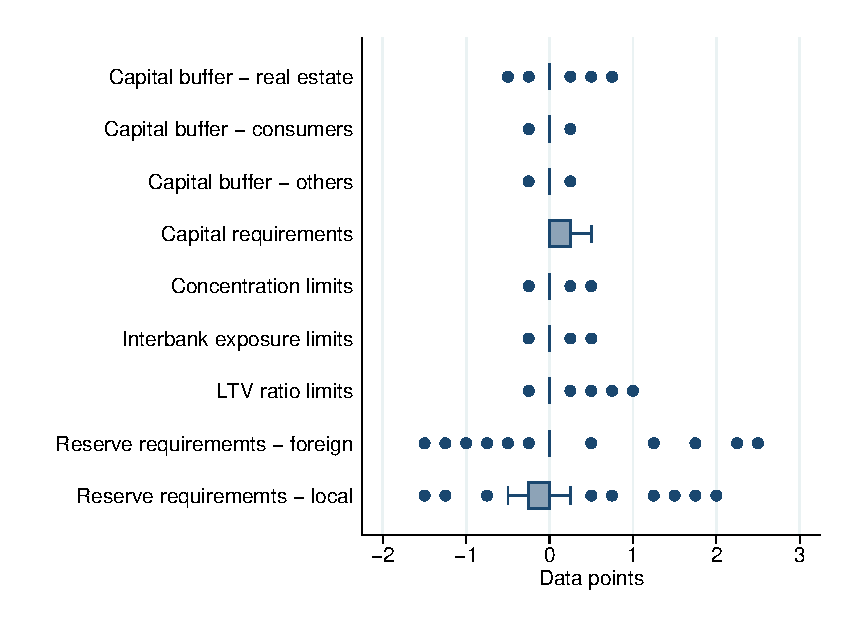
\includegraphics[scale=1.1]{C:/Users/User/work/master_thesis/analysis/output/graphs/box_plot_data.eps}
	  	\label{fig:boxplot data}
	  \end{figure}
  
	  We restrict our analysis to the following two macroprudential tools: reserve requirement on local currency and  capital requirements. First, there is an economic reason for our choice. We are interested in instruments that could affect the cost of debt of loans to firms. All capital buffers indexes are not directly related to corporate loans and most LTV changes concern housing loans. Second, only reserve requirements on local currency and capital requirements have substantial variation across time and country. Figure \ref{fig:boxplot data} plots all data points in our sample by prudential tools. Most indexes are composed of a few moves and most of the distribution mass at zero. Cross section variation within those indexes might not be enough to accurately identify their impact. The exceptions are reserve requirement on local currency and capital requirements 
	  	
 	\subsection{Firm level} \label{subsec:firm}
	Firm level data and ownership relationships are taken from the Orbis database compiled by Bureau Van Dijk.	The dataset consist of worldwide accounting and ownership information on both private and public owned companies. Ownership is considered if one firm owns at least 50\% of another firm's shares in a given year. We call the second a subsidiary firm. If a company owns one or more firms but is itself owned by another, this firm is called an intermediate and for all purposes is also considered as a subsidiary. A parent firm is the ultimate owner of a group, that is, a firm that owns one or more companies but none of its shareholders have more than 50\% of its shares.
	
	Given our identification strategy, in order to maintain a balance sample across specifications, we keep only multinationals groups, that is, corporate groups that have firms in at least two countries.  Banks, insurance and financial related companies\footnote{We keep only firms with the Orbis type identifier "C".} and firms in the utility sector\footnote{Two digit NACE codes from 35 to 39.} are also excluded since their capital structure decisions are constrained by regulation. We also exclude firms with zero or negative asset and if one of the following variables is negative: non-current liabilities, current liabilities, fixed assets, tangible assets, cash, long-term debt, loans and sales. Lastly, after constructing the leverage measures, we exclude observations where leverage is above 1. Firms with negative net worth are likely to be credit constrained and therefore not able to choose their capital structure optimally. 
	
	The final sample consists of 102,544 firms from 2008 to 2014 resulting in 461,820 firm-year observations. Table \ref{tab:number of firms} provides information on the amount of parent and subsidiary firms per host and home country in our sample. The total number of parent and subsidiary firms are 11,628 and 90,916, respectively. There are 37,682 subsidiaries for which ownership has changed during the period analyzed at least once, as shown in table \ref{tab:movers} in the appendix. Therefore column 4 double counts some firms. Also, note that we do not track the entire corporate group. For instance, there are 23,995 firms which the parent is located in countries where we do not have information. Furthermore, although we track only two firms located in Brazil, there are 120 firms in our sample that have a Brazilian parent firm.  
	
		\begin{small}
		{\setstretch{1.0}
			\begin{table}[]
\centering
\caption{My caption}
\label{my-label}
\begin{tabular}{lllll}
            & Total number & Number of    & \multicolumn{2}{l}{Number of subsidiaries} \\
            & of firms     & parent firms & by host country      & by home country     \\
Argentina   & 4            & 0            & 4                    & 1                   \\
Australia   & 406          & 42           & 364                  & 330                 \\
Austria     & 2648         & 346          & 2302                 & 3366                \\
Belgium     & 7541         & 1243         & 6298                 & 7766                \\
Brazil      & 2            & 0            & 2                    & 120                 \\
Bulgaria    & 754          & 54           & 700                  & 233                 \\
Chile       & 18           & 0            & 18                   & 23                  \\
Colombia    & 3            & 1            & 2                    & 42                  \\
Croatia     & 961          & 123          & 838                  & 459                 \\
Estonia     & 768          & 99           & 669                  & 234                 \\
Finland     & 2032         & 402          & 1630                 & 2737                \\
France      & 23215        & 1571         & 21644                & 23423               \\
Germany     & 12114        & 1549         & 10565                & 14449               \\
Greece      & 1258         & 163          & 1095                 & 786                 \\
Hungary     & 896          & 101          & 795                  & 299                 \\
Iceland     & 87           & 11           & 76                   & 213                 \\
India       & 146          & 41           & 105                  & 309                 \\
Italy       & 11535        & 1750         & 9785                 & 13070               \\
Japan       & 72           & 58           & 14                   & 2187                \\
Latvia      & 34           & 2            & 32                   & 20                  \\
Lithuania   & 2            & 0            & 2                    & 30                  \\
Luxembourg  & 435          & 71           & 364                  & 5877                \\
Malta       & 5            & 1            & 4                    & 158                 \\
Mexico      & 1            & 0            & 1                    & 133                 \\
Netherlands & 1092         & 20           & 1072                 & 6781                \\
Norway      & 5087         & 633          & 4454                 & 4454                \\
Peru        & 2            & 0            & 2                    & 4                   \\
Philippines & 40           & 1            & 39                   & 9                   \\
Poland      & 3433         & 246          & 3187                 & 618                 \\
Portugal    & 3204         & 281          & 2923                 & 1978                \\
Romania     & 2009         & 46           & 1963                 & 127                 \\
Serbia      & 533          & 22           & 511                  & 74                  \\
Slovenia    & 346          & 77           & 269                  & 395                 \\
Spain       & 11994        & 1225         & 10769                & 9345                \\
Sweden      & 9341         & 1437         & 7904                 & 11675               \\
Switzerland & 15           & 7            & 8                    & 4021                \\
Ukraine     & 511          & 5            & 506                  & 45                  \\
Others      &              &              &                      & 23995,00            \\
Total       & 102544       & 11628        & 90916                & 115791,00
\end{tabular}
\end{table}
		}
	\end{small}

	
	As highlighted in section \ref{subsec:MPI}, our macroprudential instruments indexes are not easily comparable across countries since we do not know how tight one instrument is in one country relative to the same instrument in another country. With the purpose of comparability, we index all our variables to be relative to their respective values in 2007, the year that we start tracking the prudential policies. The exception are GDP growth rate, inflation and opportunity which are growth rates and risk which is constant in time. By equalizing all variables at 2007, we can compare changes in macroprudential instruments and their association with leverage across countries (and control for other characteristics). Finally, after indexing our dataset we winsorized all firm-level variables at the 1st and 99th percentile to remove the effect of outliers (firms in which leverage has changed too strongly relative to 2007). 
	
	Figure \ref{fig:time graph} illustrate our variables transformation. Each plot has the yearly average of financial leverage across all firms in the sample (rescaled to start at zero in 2007) and one of the macroprudential policy indexes. By construction, in 2007 all variables have the same value. We see that leverage increase slightly with time and most instruments were tightened apart from reserve requirements on local currency.   
	
		\begin{figure}[h!]
		\centering
		\caption{Average of macroprudential policies indexes in time}
		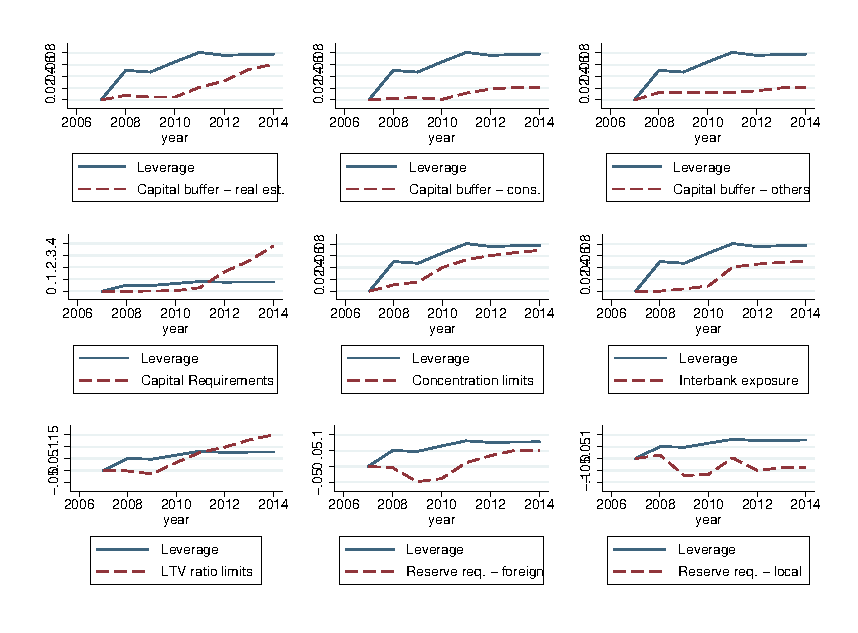
\includegraphics[scale=1.1]{C:/Users/User/work/master_thesis/analysis/output/graphs/time_graphs.eps}
		\label{fig:time graph}
	\end{figure}
	
	Statistics on firm level data are summarized in panels A and B of table \ref{tab:number of firms}. Financial leverage is defined as the ratio of total non-equity liabilities to total assets. Reserve req. spillover and capital requirements spillover are, respective, $\beta_{2,rr}$ and $\beta_{2,cr}$ as described in section \ref{sec:strategy}. Among the control variables tangibility is construct as the ratio of fixed assets to total assets. While tangible assets can be used as collateral, implying a positive relationship between tangibility and leverage, the depreciation of fixed assets reduces taxable income. Hence, tangible assets can also be substitute to debt as tax shield. We use the logarithm of fixed assets to proxy for firm size, which is expected to be positively associated to leverage. Profitability is the ratio of earning before interest, tax, depreciation and amortization (EBITDA) to total assets. Higher profits may facilitate access to credit but firms with larger cash flow may also opt to finance themselves with retained earnings as predicted by the pecking order theory of capital structure. Thus, the relationship between profitability and leverage is ambiguous. Opportunity is the median annual growth rate of sales in an industry in a particular country. We expect this variable to be positive associated to leverage as higher growth opportunities signal future profits that can be used to increase the ability to borrow in the present. 
	   
		\begin{small}
		{\setstretch{1.0}
			\begin{table}[htbp]\centering
\def\sym#1{\ifmmode^{#1}\else\(^{#1}\)\fi}
\caption{Summary statistics of firm level variables}
\begin{tabular}{l*{1}{ccccc}}
\hline\hline
                    &\multicolumn{5}{c}{}                                            \\
                    &       count&        mean&          sd&         min&         max\\
\hline
Financial leverage  &      492166&        0.59&        0.27&        0.00&        1.00\\
Adjusted financial leverage&      343359&        0.52&        0.28&        0.00&        1.00\\
Debt leverage       &      431856&        0.12&        0.19&        0.00&        1.00\\
Long term debt      &      441916&        0.07&        0.15&        0.00&        1.00\\
Short term debt     &      471801&        0.05&        0.11&        0.00&        1.00\\
Overall capital strigency&       66078&        7.36&        1.21&        4.00&       10.00\\
Initial capital stringency&       66078&        5.45&        1.09&        2.00&        7.00\\
Capital regulatory index&       66078&        1.91&        0.53&        1.00&        3.00\\
Tax rate            &      492149&        0.54&        0.11&        0.18&        1.37\\
Overall capital strigency spillover&      492166&        0.05&        0.49&       -5.65&        6.00\\
Initial capital stringency spillover&      492166&        0.03&        0.42&       -4.79&        4.82\\
Capital regulatory index spillover&      492166&        0.01&        0.17&       -2.00&        2.00\\
Tax rate spillover  &      492166&        0.02&        0.10&       -0.52&        0.70\\
Tangibility         &      492166&        0.32&        0.29&        0.00&        1.00\\
Log of fixed assets &      492166&       14.52&        2.69&        4.32&       18.30\\
Profitability       &      492166&        0.09&        0.17&       -1.96&        1.28\\
Opportunity         &      492166&       -0.03&        0.09&       -0.33&        0.22\\
Risk                &      492166&        0.09&        0.17&        0.00&        3.30\\
Inflation rate      &      492124&        0.02&        0.02&       -0.01&        0.22\\
GDP growth rate     &      492166&        0.00&        0.03&       -0.15&        0.10\\
Private credit to GDP&      492148&        1.00&        0.32&        0.12&        1.98\\
Policy rate         &      451067&        1.40&        1.19&        0.02&       12.54\\
Political Risk      &      492166&       77.85&        7.07&       52.00&       92.50\\
Exchange rate risk  &      492166&        9.47&        0.90&        1.00&       10.00\\
Law and order       &      492166&        4.97&        0.65&        2.00&        6.00\\
\hline\hline
\end{tabular}
\end{table}

		}
	\end{small}

Last but not least, risk is the standard deviation of firms' profitability over the sample period and it is our proxy for the riskiness of firms. Results concerning the relationship between leverage and business risk are ambiguous. Among the authors, \cite*{bradley1984existence} find a negative association, \cite*{bennett1993determinants} a positive, \cite*{kale1991effect} suggest a U-shape relationship and \cite{titman1988determinants} argue in favor of no relationship between business risk and leverage. We differ from previous studies by separating the supply from the demand effect of firms' riskiness on capital structure. On one hand, we expect riskier firms to have higher leverage.  Managers, acting on behalf of shareholders, favor financing risky projects with debt, as the risk is shared among stockholders and creditors while the gains are limited to the latter. On the other hand, the interaction of earnings' volatility and the macroprudential policies indexes are expected to be negatively associated to leverage, as volatility increases the cost of accessing external capital (\cite{minton1999impact}).

	%As an alternative measure, adjusted tangibility is the ratio of tangible fixed assets to total assets. 
	%%Growth opportunities is BLA BLA
	%Adjusted financial leverage is a similar measure but subtracting cash and equivalent from both the numerator and the denominator. 
	\subsection{Country level} \label{subsec:country}
	Panel C of Table \ref{tab:number of firms} provides statistics at the country level. We control for political risk, exchange rate risk and law and order using the indexes from the \textit{International Country Risk Guide}. We inverted the original risk indexes, resulting in higher scores indicating greater risk. \cite*{kesternich2010afraid} find that political risk can both increase or decrease firm leverage. A more unstable political environment may discourage banks to provide loans, but parent firms might want to reduce their value at risk by leveraging their subsidiaries' operations. \cite*{burgman1996empirical} studies determinants of capital structure that differ between domestic and multinational corporations, finding political and exchange rate risk to be positively associated with leverage. The index for law and order proxy for the institutional level, which \cite*{demirgucc1998law} show to affect firms debt growth. Higher scores mean greater juridical strength.
	
	 We include four macro controls from the \textit{World Development Indicators} database from the World bank. Private credit to GDP is the share of credit to the private sector to GDP and is a proxy to financial development. We expect financial development to affect leverage positively. Inflation is the annual log change in the consumer price index. As \cite{huizinga2008capital} point out, an inflationary environment may discourage firms to borrow as risk premiums increase. GDP growth rate is the annual growth rate of GDP. Credit markets are pro-cyclical, so we expect a positive coefficient between GDP growth and leverage. Lastly, we include the policy rate of each country from IMF's International Financial Statistics. \cite*{jimenez2012credit} show that tight monetary policy reduces bank lending. Thus, the relationship between policy rate and leverage is expected to be negative. Descriptions and sources of all variables are displayed in table \ref{tab:definition} in the appendix.
			
	\section{Empirical strategy and hypotheses}
	\label{sec:strategy}
	Equation \ref{eq:optimal leverage in theory} from section \ref{subsec:opt_leverage} provides the theoretical foundation for our empirical models. We start with a specification that allow us to estimate all the effects of the model on leverage: 
	\begin{equation}
	\begin{aligned}
	\lambda_{imc(i),t}=&\alpha_0\tau_{c(i),t}+\beta_0\Pi_{c(i),t}+\beta_1\tau_{c(i),t}\Pi_{c(i),t}\\
	&+\alpha_1\sum_{j=1}^{n}(\tau_{c(i),t}-\tau_{c(j),t})\rho_{j,t}+\beta_2\sum_{j=1}^{n}(\Pi_{c(i),t}-\Pi_{c(j),t})\rho_{j,t}\\
	&+\Gamma_1 X_{i,t}+\Gamma_2 X_{c(i),t}+f_{m}+f_{t}+\varepsilon_{i,t},
	\label{eq:optimal leverage empirically 1}
	\end{aligned}
	\end{equation}
	
	where $i$ denotes firm (either subsidiary or parent), $m$ the multinational (indexed by the parent firm) and $t$ the year. $c(i)$ stands for the country where firm $i$ is hosted. For example, $\tau_{c(i),t}$ represents the effective tax rate in the country where firm $i$ is hosted. The dependent variable is a financial leverage measure of the firm. $\Pi_{i,t}$ is the vector of indexes for macroprudential instruments used in the host country. $\rho_{j,t}$ is the asset share of firm $j$ within the multinational group. $f_{m}$ and $f_{t}$ are respectively the multinational and time fixed effects. $X_{i,t}$ and $X_{c(i),t}$ are the set of firm- and country-level control variables, respectively. We also include the corporate tax level at the host country $\tau_{c(i),t}$, the tax incentive to shift debt, and the interaction between tax and macroprudential policies. Note, that we abstract from the last term of equation \ref{eq:optimal leverage in theory}. 
	
	However, if our intention is to find causal relationship between macroprudential policies and capital structure, model \ref{eq:optimal leverage empirically 1} might not be robust enough. Macroprudential instruments can be correlated to other factors at the country level that could impact the supply of credit to firms. The inclusion of country-level variables helps to mitigate those identification concerns but it might not be sufficient. In order to address this, we rely on the variation within multinationals and perform the following model:
	
	\begin{equation}
	\begin{aligned}
	\lambda_{imc(i),t}=&\alpha_1\sum_{j=1}^{n}(\tau_{c(i),t}-\tau_{c(j),t})\rho_{j,t}+\beta_2\sum_{j=1}^{n}(\Pi_{c(i),t}-\Pi_{c(j),t})\rho_{j,t}\\
	&+\beta_3Risk_{i}\Pi_{c(i),t}+\Gamma_1 X_{i,t}+f_{c(i),t}+f_{m}+\varepsilon_{i,t}.
	\label{eq:optimal leverage empirically 2}
	\end{aligned}
	\end{equation}
	
	In this model we include country*year fixed effects ($f_{c(i),t}$) to account for unobservable characteristics that could be driving the supply effects rather than macroprudential policies. All country-time specific variables cannot be included in this specification. In order to study the domestic impact we interact both macroprudential indexes with our proxy of firms' riskiness, their volatility of EBITDA in the sample period ($Risk_{i}$). We keep the multinatinal $f_{m}$ fixed effects and firm-level control variables.  
	
	Still, a complete causal relationship cannot be inferred by performing regression \ref{eq:optimal leverage empirically 2}. On the basis of demand factors alone, the optimal leverage level does not have to be constant in time. Consequently, multinational fixed effects might not account for all the unobservable characteristics that could be driving the demand side. The inclusion of year fixed effects is not sufficient since it does not capture cross-firm unobservable variability.  
	
	According to the model developed in section \ref{sec:model}, the capital structure decision is taken at the multinational level. Hence, we can push further our identification strategy towards accounting all the demand factors of leverage. By tracking multinationals composed of firms hosted at different countries exposed to cross-country and time varying macroprudential policies we can control for unobservables characteristics of every multinational group at each year as follows:   
	
	\begin{equation}
	\begin{aligned}
	\lambda_{imc(i),t}=&\beta_3Risk_{i}\Pi_{c(i),t}+\Gamma_1 X_{i,t}+f_{m,t}+f_{c(i),t}+\varepsilon_{i,t}.
	\label{eq:optimal leverage empirically 3}
	\end{aligned}
	\end{equation}
	
	The model includes multinational*year ($f_{m,t}$) and country*year ($f_{c(i),t}$) fixed effect, besides the interaction of macroprudential indexes with firms' riskiness and firm-level controls. The drawback of this specification is that we have to drop the international effect variables. 		
	
		\subsection{Hypotheses}
	\label{subsec:hypothesis} 
	 For the reasons elucidated in section \ref{subsec:MPI}, we restrict our analysis to the impact of reserve and capital requirements on financial leverage. Both instruments are expected to be positively correlated to banks' cost of providing loans ($\phi_{rr}>0$ and $\phi_{cr}>0$) as banks need to hold more capital and reserves for the amount of loans provided. Given expression \ref{eq:phi vector} and equation 	\ref{eq:optimal leverage in theory} our hypotheses on the parameters of models \ref{eq:optimal leverage empirically 1}, \ref{eq:optimal leverage empirically 2} and \ref{eq:optimal leverage empirically 3} can be stated as follows:

	\begin{hyp}[H\ref{hyp:H1}] \label{hyp:H1}
		holding everything else constant and considering only the domestic effect through the cost of debt ($\beta_{0}$), a tightening/loosening in reserve and capital requirements reduces/increases firms' financial leverage ($\beta_{0,rr}<0$, $\beta_{0,cr}<0$).
	\end{hyp}
	\begin{hyp}[H\ref{hyp:H2}] \label{hyp:H2}
		holding everything else constant the riskiness of the firm and the incentive to shift debt within a multinational reinforce the effects described in hypothesis \ref{hyp:H1}. 
	\end{hyp}
Note that the equation \ref{eq:optimal leverage in theory} implies $\beta_{1}=-\beta_{0}$, that is, the coefficient of the effect of macroprudential policies through higher tax shields will have the same magnitude but opposite sign to the coefficient of the effect via higher interest payments. Consequently, from hypothesis \ref{hyp:H1} we expect $\beta_{1}>0$. 
	 
	\section{Results} \label{sec:result}
	 Table \ref{reg:benchmark} presents the results of our empirical strategy described in section \ref{sec:strategy}. The dependent variable is financial leverage. Column 1 reports the estimates of equation \ref{eq:optimal leverage empirically 1}. Besides the set of variables related to macroprudential and tax (spillovers and interactions) the regression includes firm-, country-level controls, multinational and year fixed effects. The first four lines are related to hypothesis \ref{hyp:H1}. The signs are as expected but only the effects of capital requirement are statistically significant at 5\%. Considering the average tax level relative to 2007 in our sample (0.96) a tightening in capital requirements (0.25) is associated with leverage being -0.266*0.25 + 0.96*0.308*0.25 = 0.7\% higher on average. The effect capital requirements on tax shields dominates in this example.   
	 
	 	\begin{small}
	 	{\setstretch{1.0}
	 		\begin{longtable}{lccc}\\
	\label{reg:benchmark}\\
	\multicolumn{4}{c}{Table \ref{reg:benchmark} - Regression results, macroprudential policies and capital structure }\\
		\multicolumn{4}{c}{(\textit{Dependent variable}: financial leverage)}
	\\ \hline \hline
	Model & (1) & (2) & (3)  \\ \hline
	 &  &  &  \\ \endfirsthead
\multicolumn{4}{c}{Table \ref{reg:benchmark} - Regression results, macroprudential policies and capital structure }\\
\multicolumn{4}{c}{(\textit{Dependent variable}: financial leverage)\textit{(Continued)}}
\\ \hline \hline
Model & (1) & (2) & (3)  \\ \hline 
 &  &  &  \\ \endhead
  \hline
  \multicolumn{4}{r}{{\textit{(Continued)}}}\\ \endfoot

 \endlastfoot
 Effects of macroprudential policies  &  &  &  \\
\quad Reserve req. on local currency ($\beta_{0,rr}$) & 0.095 &  &  \\
 & (0.083) &  &  \\
\quad Capital requirement ($\beta_{0,cr}$) & -0.266** &  &  \\
 & (0.124) &  &  \\

\quad Reserve req. on local currency*tax ($\beta_{1,rr}$) & -0.016 &  &  \\
 & (0.080) &  &  \\
\quad Capital requirement*tax ($\beta_{1,cr}$)& 0.308** &  &  \\
 & (0.127) &  &  \\

\quad Reserve req. on local currency spillover ($\beta_{2,rr}$) & -0.071** & -0.056** &  \\
 & (0.028) & (0.027) &  \\
\quad Capital requirement spillover ($\beta_{2,cr}$) & -0.025 & -0.015 &  \\
 & (0.027) & (0.026) &  \\

\quad Reserve req. on local currency*risk ($\beta_{3,rr}$) &  & -0.322** & -0.337* \\
 &  & (0.157) & (0.172) \\
\quad Capital requirement*risk ($\beta_{3,cr}$) &  & -0.250** & -0.399*** \\
 &  & (0.123) & (0.140) \\
 Effects of corporate tax &  &  &  \\
\quad Tax rate ($\alpha_{0}$) & 0.095** &  &  \\
 & (0.042) &  &  \\
\quad Tax rate spillover ($\alpha_{1}$) & 0.015 & -0.014 &  \\
 & (0.030) & (0.045) &  \\
  Firm characteristics &  &  &  \\
\quad Tangibility & -0.013*** & -0.013*** & -0.014*** \\
 & (0.002) & (0.002) & (0.003) \\
\quad Log of fixed assets & 0.880*** & 0.892*** & 0.947*** \\
 & (0.064) & (0.062) & (0.068) \\
\quad Profitability & -0.004*** & -0.004*** & -0.004*** \\
 & (0.001) & (0.001) & (0.001) \\
\quad Opportunity & 0.111*** & 0.106*** & 0.148*** \\
 & (0.019) & (0.022) & (0.031) \\
\quad Risk & 0.081*** & 0.105*** & 0.121*** \\
 & (0.022) & (0.023) & (0.024) \\
   Macroeconomic controls &  &  &  \\
\quad Inflation & 0.060 &  &  \\
 & (0.180) &  &  \\
\quad GDP growth rate & 0.142 &  &  \\
 & (0.105) &  &  \\
\quad Private credit to GDP & 0.032 &  &  \\
 & (0.027) &  &  \\
\quad Policy rate & -0.070** &  &  \\
 & (0.033) &  &  \\
\quad Political Risk & -0.076 &  &  \\
 & (0.068) &  &  \\
\quad Exchange rate risk & -0.119*** &  &  \\
 & (0.020) &  &  \\
\quad Law and order & 2.533* &  &  \\
 & (1.299) &  &  \\
 &  &  &  \\
Observations & 417,845 & 455,053 & 406,332 \\
Number of multinationals & 27,460 & 29,453 & 19,044 \\
Year fixed effects & Yes & No & No \\
Multinational fixed effects & Yes & Yes & No \\
Country*year fixed effects & No & Yes & Yes \\
 Multinational*year fixed effects & No & No & Yes \\ \hline
\multicolumn{4}{c}{ Robust standard errors in parentheses} \\
\multicolumn{4}{c}{ *** p$<$0.01, ** p$<$0.05, * p$<$0.1} \\
\end{longtable}

	 	}
	 \end{small}
 
	Evidence supporting hypothesis \ref{hyp:H2} is found only for reserve requirement on local currency. As \cite{buch2017cross} note, many capital requirement regulations were implemented on the basis of international agreements, potentially limiting spillover. To illustrate the effect, we consider a multinational firm that consists of the parent firm and one subsidiary with assets of equal size. A tightening on the reserve requirements on local currency in the country of the subsidiary is associated with a spillover to the parent firm that reduces financial leverage by 0.09\% (the estimated coefficient, -0.071, times the  asset share of the parent firm, 0.5, times the tightening, 0.25). Overall, the results suggest that firms respond locally to changes in capital requirements while multinationals have an extra incentive to shift debt due to moves in reserve requirements on local currency.
	 
	 The coefficient for corporate tax rate is estimated to be 0.095 and statistically significant at 5\%. Considering  capital requirements one measure tighter relative to 2007 (0.25), an increase in the effective tax rate by 0.08 (one standard deviation) is associated, on average, with 0.08*0.095 + 0.08*0.25*0.308 = 1.4\% higher leverage\footnote{\cite{huizinga2008capital} find the domestic effect of one standard deviation higher corporate tax on leverage to be 1.0\% while the total effect, including tax incentive to shift debt, to be 1.4\%.}. We cannot reject the corporate tax spillover's coefficient being equal to zero. Among the control variables, tangibility and profitability have significant negative coefficients at 1\%. The substitution effect seems to dominate on average in our sample for both variables. Next, as expected, log of fixed assets, opportunity and risk have positive and statistically significant at 1\% estimated coefficients. Exchange rate risk, policy rate and law and order enter the regression with expected sign at 1\%, 5\% and 10\% significance level, respectively. Other macroeconomic control variables are statistically insignificant.
	 
	 As highlighted in section \ref{sec:strategy}, the results in column 1 of table \ref{reg:benchmark} do not imply causality since we cannot disentangle macroprudential policies variation from other shocks that we do not observe that are common to firms hosted in the same country. In equation \ref{eq:optimal leverage empirically 2} we include country*year fixed effects to account for any variation at the country-level for each year. Consequently, in this specification we have to drop the macroprudential indexes and their interaction with tax rates. The number of observations increase to 455,053 from 417,845 as firms with missing country-level variables enter the sample. To test the domestic effect we introduce an interaction term between each of the macroprudential indexes and our proxy of firms' riskiness. So far we have assumed the cost of debt to be homogeneous across firms hosted in the same country. However, we expect the interest rate charged on loans to be higher for riskier firms. The results of the estimation support hypothesis \ref{hyp:H2}. With the exception of spillover from capital requirements, all coefficients are negative and significant at 5\% level. All firm controls remain with expected sign and significant at 1\% while, again, no evidence is found of tax incentive to shift debt.
	 
	  The specifications in columns 1 and 2 still miss time variation within each multinational that could be associated to the cost of debt and driving the results (for example, changes in bank relationship or management strategy). To this purpose, we estimate model \ref{eq:optimal leverage empirically 3} which account for unobservables at the multinational level for every year in our sample. The results are shown in column 3 of table \ref{reg:benchmark}. Note that with this specification, by construction, the parameters related to international spillover cannot be included in the model. Once multinational*year fixed effects are introduced, the spillover coefficients simply reflect the domestic effect (which in turn is collinear with country*year fixed effects). The number of observations decrease to 406,332 as some multinationals with common prudential tightening stance across host countries at a given year have to be dropped.
	  
	   Accounting for unobservables at the multinational level for every year reinforces our hypotheses. First, the magnitude and significance of capital requirements domestic effect are greater than the model with time invariant multinational fixed effect. To illustrate, considering the average risk level in our sample (0.09) the domestic effect of a increase in capital requirements is estimated to lower leverage by -0.399*0.09 = 3.6\% on average, a sizable impact given that the average leverage level in our sample is 7\% higher than the level in 2007. increase Reserve requirements on local currency appears with negative sign but significant only at 10\% level. Firm-level controls remain statistically significant and with the expected signs. 
	  
	\section{Robustness tests and extensions} \label{sec:robustness}
	Table \ref{reg:alternative} show that our results depend on the choice of leverage measure used. We present estimates of equation \ref{eq:optimal leverage empirically 2} for alternative leverage measures in order to check both the domestic and the international effects. In column 1 we adjust our financial leverage measure by subtracting cash and cash equivalents from total non-equity liabilities and from total assets. This adjustment reflect that firms may hold cash to pay off existing debt. In this model, we observe a significant association of reserve requirement and leverage and none between the latter and capital requirements. \cite*{sanchez2013corporations} report a upward trend in cash holdings by U.S. corporations following the financial crisis in 2008. If we expect the same trend to firms globally, then perhaps the capital requirements index is simply capturing how cash holdings affect leverage.  
	
	Long-term debt to total assets is considered in column 2 of table \ref{reg:alternative}. International spillover appears to not impact decisions regarding long-term debt while the domestic effect is significant at 1\% for both indexes. Our model predicts that the impact of macroprudential policies to firms' leverage is transmitted through the bank sector, that is, banking loans. Therefore, the positive sign for the domestic effects in column 2 suggest that firms may substitute banking loans with long-term debt, as the cost of debt of the former increases with tighter macroprudential policies. 
	
	\begin{small}
	{\setstretch{1.0}
		\begin{tabular}{lccccc}
\multicolumn{6}{c}{Effect of macroprudential policies on firm's financial leverage: alternative measures} \\ \hline
 & (1) & (2) & (3) & (4) & (5) \\
 & Financial & Adjusted & Debt & Long-term & Short-term \\
VARIABLES & leverage & leverage & leverage & debt & debt \\ \hline
 &  &  &  &  &  \\
Reserve req. on local currency & -0.330* & -0.539** & -1.687*** & -1.129** & -0.346 \\
 & (0.179) & (0.244) & (0.436) & (0.461) & (0.528) \\
LTV ratio limits & 0.068 & -0.694 & -0.502 & -0.534 & 0.839 \\
 & (0.299) & (0.449) & (0.834) & (0.880) & (0.979) \\
Capital requirement & -0.544*** & -0.285 & 0.638 & 0.744 & 0.577 \\
 & (0.198) & (0.254) & (0.516) & (0.598) & (0.617) \\
Capital buffer - real estate & 0.938** & 0.996* & 4.540*** & 4.788*** & 0.742 \\
 & (0.413) & (0.580) & (1.010) & (1.113) & (1.231) \\
Reserve req. on local currency*tax & 0.375** & 0.356 & 1.890*** & 1.429*** & 0.525 \\
 & (0.183) & (0.241) & (0.436) & (0.457) & (0.528) \\
LTV ratio limits*tax & -0.057 & 0.778* & 0.088 & -0.031 & -1.016 \\
 & (0.313) & (0.470) & (0.868) & (0.912) & (1.032) \\
Capital requirement*tax & 0.596*** & 0.337 & -0.405 & -0.425 & -0.757 \\
 & (0.205) & (0.266) & (0.538) & (0.625) & (0.647) \\
Capital buffer - real estate*tax & -1.039** & -0.783 & -5.058*** & -5.072*** & -1.488 \\
 & (0.435) & (0.608) & (1.050) & (1.154) & (1.277) \\
Tax rate & 0.197** & 0.319*** & 1.966*** & 1.556*** & 0.802*** \\
 & (0.081) & (0.104) & (0.224) & (0.259) & (0.271) \\
 &  &  &  &  &  \\
Observations & 828,172 & 638,383 & 552,167 & 363,643 & 427,562 \\
R-squared & 0.32 & 0.33 & 0.36 & 0.41 & 0.36 \\
Number of firms & 173,322 & 143,443 & 113,986 & 76,316 & 85,378 \\
Industry fixed effects & Yes & Yes & Yes & Yes & Yes \\
 Multinational*year fixed effects & Yes & Yes & Yes & Yes & Yes \\ \hline
\multicolumn{6}{c}{ Robust standard errors in parentheses} \\
\multicolumn{6}{c}{ *** p$<$0.01, ** p$<$0.05, * p$<$0.1} \\
\end{tabular}

	}
\end{small}

Column 3 of table \ref{reg:alternative} shows the results for short-term to total assets as dependent variable. The interaction term between capital requirements and risk gain the expected negative sign in line with the result in table \ref{reg:alternative} (column 2). The coefficient of reserve requirements on local currency spillover has the opposite sign to what we expect. However, in our model we do not account for internal capital market. This result may be driven by multinationals using short term debt through internal capital market to shift debt across subsidiaries. Hence, if external funding is relative costly to a subsidiary, firms hosted in countries with better borrowing conditions can lend to former. 

Table \ref{reg:extension} presents other robustness checks to our model. In all columns we regress equation \ref{eq:optimal leverage empirically 3} which we believe to be the most robust. First, introducing a separation between spillover to the parent firm versus other subsidiaries do not change our results. The domestic effects of macroprudential policies on financial leverage remain with the expected sign and significant. No evidence of international spillover on financial leverage is found. Second, we include industry fixed effects in order to control for sector-specific drivers that our firm-level variables might not account for. The coefficient for the interaction between capital requirements and risk is now significant at 5\% level while the parameter of reserve requirements on local currency interacted with risk is not significant different to zero. Finally,  column 3 shows the results of the estimation of a capital structure partial adjustment model. Our results are not robust to the inclusion of a lag of the dependent variable. 

	\begin{small}
	{\setstretch{1.0}
		\begin{tabular}{lccc}
\multicolumn{4}{c}{Effect of macroprudential policies on firm's financial leverage} \\ \hline
 & (1) & (2) & (3) \\
 & Shifting to & Sector & Sector \\
 & parent versus & fixed & fixed \\
VARIABLES & other firms & effects & effects \\ \hline
 &  &  &  \\
lag\_leverage &  &  & 0.883*** \\
 &  &  & (0.005) \\
Reserve req. on local currency*risk & -0.338** & -0.304 & 0.018 \\
 & (0.172) & (0.192) & (0.073) \\
Capital requirement*risk & -0.398*** & -0.345** & -0.129 \\
 & (0.141) & (0.155) & (0.085) \\
Reserve req. on local currency spillover to parent & 0.070 &  &  \\
 & (0.159) &  &  \\
Reserve req. on local currency spillover to other subsidiaries & 0.120 &  &  \\
 & (0.146) &  &  \\
Capital requirement spillover to parent & -0.008 &  &  \\
 & (0.139) &  &  \\
Capital requirement spillover to other subsidiaries & -0.075 &  &  \\
 & (0.101) &  &  \\
Tax rate spillover to parent & -5.366 &  &  \\
 & (4.141) &  &  \\
Tax rate spillover to other subsidiaries & -5.385 &  &  \\
 & (4.133) &  &  \\
Tangibility & -0.014*** & -0.013*** & -0.005*** \\
 & (0.003) & (0.003) & (0.001) \\
Log of fixed assets & 0.947*** & 0.897*** & 0.260*** \\
 & (0.068) & (0.069) & (0.024) \\
Profitability & -0.004*** & -0.004*** & -0.002*** \\
 & (0.001) & (0.001) & (0.000) \\
Opportunity & 0.147*** & 0.047* & 0.042** \\
 & (0.031) & (0.028) & (0.021) \\
Risk & 0.121*** & 0.151*** & 0.087*** \\
 & (0.024) & (0.025) & (0.020) \\
 &  &  &  \\
Observations & 406,332 & 402,240 & 315,396 \\
Number of multinationals & 19,044 & 18,810 & 16,243 \\
Multinational fixed effects & Yes & Yes & Yes \\
 Country*year fixed effects & Yes & Yes & Yes \\ \hline
\multicolumn{4}{c}{ Robust standard errors in parentheses} \\
\multicolumn{4}{c}{ *** p$<$0.01, ** p$<$0.05, * p$<$0.1} \\
\end{tabular}

	}
\end{small}
	
% Tangibility appears with a positive coefficient, suggesting that the effect of fixed assets as collateral dominates the substitution effect due to depreciation. Inflation is negatively associated to long-term debt. As \cite{huizinga2008capital} points out, in an inflationary environments the uncertainty about ex-post real interest rate may inhibit leverage on long-term liabilities. In all specifications, tax rate coefficients are significantly at 1\% and has a negative sign. Surprisingly, the tax incentive to shift debt is statistically significantly at 5\% and positive for nine out of 12 specifications.
	
%Tangibility regained the negative sign, suggesting that the substitution effect coming from the depreciation tax shield matters more when deciding to finance through short-term loans. 

%\subsection{Alternative models} \label{subsec:alt_models}

	\section{Conclusion} \label{sec:conclusion}
		
	This paper shows that firms' capital structure are sensitive to macroprudential policies, specifically capital and reserve requirements. We propose a simple theoretical model  where changes in macroprudential instruments impact banks' cost of providing loans that ultimately are transmitted to firms via their cost of debt. Using data from multinationals in 37 countries from 2008 to 2014 we are able to identify this transmission channel since the data allow us to control for unobservable factors on the demand side and shocks at the country-level that could be correlated to leverage and macroprudential policies. Therefore, we use the cross-country variation in capital and reserve requirements across subsidiaries within one multinational to identify their effects on capital structure. Our model also predicts macroprudential policies' effects from one country to spillover to firms hosted at others, as multinationals will take advantage of differences in credit conditions (and tax rates) to allocate debt across subsidiaries. 
	
	Overall, the results suggest that firms respond locally to changes in capital requirements while multinationals have an extra incentive to shift debt due to moves in reserve requirements. Moreover, the risk of firms appears to enhance the domestic effect, as riskier firms tend to face worse credit conditions relative to their safer counterparts. Hence, macroprudential instruments are effective in curbing excessive leverage and their effect are stronger to firms more likely to experience shortfall in cash-flow. In our analysis, the most significant effect comes from capital requirements, that in the period were only tightened. Hence, we only capture one side of the effect. An interesting extension to our work is to study if this interaction effect is asymmetric, that is, whether tightening and loosening in macroprudential policies affect risky firms with the same intensity.
	
		
	\clearpage
	
	\singlespacing
	\bibliography{C:/Users/User/work/master_thesis/analysis/code/text/bibliography/references}
	\bibliographystyle{C:/Users/User/work/master_thesis/analysis/code/text/bibliography/te}
	
	
	
%	\clearpage
	
%	\onehalfspacing
	

	
	\clearpage
	
\section*{Appendix } 
\label{sec:appendixa}
	\addcontentsline{toc}{section}{Appendix A}
	
	\begin{small}
	{\setstretch{1.0}
		  \begin{longtable}{cc}\\
  	\label{tab:movers}\\
  	\multicolumn{2}{c}{Table \ref{tab:movers} - Number of firms that }\\
  		\multicolumn{2}{c}{changed ownership}\\ \hline \hline
            &\multicolumn{1}{c}{Movers}\\
\hline
1           &       27,990\\
2           &        7,544\\
3           &        1,783\\
4           &         314\\
5           &          50\\
6           &           1\\
\hline
Total       &       37,682\\
\hline
\end{longtable}
	}
\end{small}

	\begin{small}
	{\setstretch{1.0}
		% Please add the following required packages to your document preamble:
% \usepackage{graphicx}
%\begin{longtable}[]
	\centering
	%\resizebox{\textwidth}{!}{%
		\begin{longtable}{p{2.5in}p{4in}p{2in}}
				\label{tab:definition}\\
			\multicolumn{3}{c}{Table \ref{tab:definition} - Variable definitions and data sources}\\
			\hline 
			Variable      & Definition & Source \\
			\hline \endfirsthead
			
				\multicolumn{3}{c}{Table \ref{tab:definition} - Variable definitions and data sources \textit{(Continued)}}\\
			\hline 
			Variable      & Definition & Source \\
			\hline \endhead
			
			\hline
			\multicolumn{3}{r}{{\textit{Continued}}}\\ 
			\endfoot
			\hline
			\endlastfoot
			Financial leverage      & Ratio of non-equity liabilities to total assets & Orbis \\
		
		Restriction on banking activities & Index for the extent to which banks may engage in securities, insurance and real estate activities(higher values indicate more restrictive) & \cite{barth2013bank}\\
			
			Financial conglomerates restrictiveness & Index for restrictions on banks' ownership of nonfinancial firms and on non-bank firms owning banks (higher values indicate more restrictive) & \cite{barth2013bank}\\	
			
			Capital regulatory stringency & Index measuring stringency in capital requirements (higher values indicate higher stringency) & \cite{barth2013bank}\\
			
			Official supervisory power & Index capturing whether the supervisory authorities have the authority to take specific actions to prevent and correct problems (higher values indicate greater power) & \cite{barth2013bank}\\	
			
				External governance & Index for the quality and presence of certain accounting practices, financial statement transparency, external rating and auditing  (Higher values indicate better corporate governance) & \cite{barth2013bank}\\
			
			Restriction on banking activities spillover & Sum of restriction on banking activities index differences weighted by local asset shares & \cite{barth2013bank}\\
			
			Financial conglomerates restrictiveness spillover & Sum of Financial conglomerates restrictiveness index  differences weighted by local asset shares & \cite{barth2013bank}\\	
			
			Capital regulatory stringency spillover & Sum of capital regulatory stringency index differences weighted by local asset shares & \cite{barth2013bank}\\
			
			Official supervisory power spillover & Sum of official supervisory power index differences weighted by local asset shares & \cite{barth2013bank}\\	
			
			External governance spillover & Sum of external governance index differences weighted by local asset shares & \cite{barth2013bank}\\
				
			Tax rate & Taxes and other mandatory contributions after accounting  for deductions and exemptions to total commercial profit & World Bank Doing Business indicators\\
			Tax rate spillover & Sum of international corporate tax rate  differences weighted by local asset shares& World Bank Doing Business indicators\\
			Tangibility& Ratio of fixed assets to total assets & Orbis\\
			Log of fixed assets& logarithm of fixed assets & Orbis\\
			Profitability& Ratio of EBITDA to total assets & Orbis\\
			Risk & Standard deviation of the firm's ratio of EBITDA to total assets over the period 2008-2014& Orbis\\
			Opportunity & Median of the annual growth rate of sales per country and industry& Orbis\\
			Private credit to GDP & Ratio of credit to the private sector to GDP & World Bank indicators\\	
			Inflation & Annual log change in the CPI & World Bank indicators\\
			GDP growth rate &Annual percentage change in the GDP & World Bank indicators\\
			 Policy rate &Central Bank Policy Rate, Percent per annum & IMF International Financial Statistics \\
			Exchange rate risk &Annual (December) index of exchange rate risk &International Country Risk Guide\\
			Law and order &Annual (December) index of law and order &International Country Risk Guide\\
			Political risk &Annual (December) index of political risk &International Country Risk Guide\\
		\end{longtable}%
	%}
%\end{longtable}
	}
\end{small}

\end{document} 